\chapter{Summary, Discussion, \& Conclusion} \label{ch:conclusion}

\section{Chapter Purpose \& Structure}

This chapter has two purposes. The first is to review the previous chapters and summarize the contributions presented in each. This is the focus of Section \ref{sec:summary}. The second purpose is to supply an answer to Research Question 3:

\blockquote{What steps are necessary to establish \acf{evdt} as a continually development framework, a community of practice, and a growing code repository?}

Responding to this research question is the focus of Section \ref{sec:future-inquiry}, which provides Research Deliverables 3a and 3b:

	\begin{enumerate}[label=\emph{\alph*},itemsep=0pt,parsep=0pt]
		\item{An assessment of lessons learned from these \acf{dss} development processes} 
		\item{An outline of potential future \ac{evdt} refinement and extension, such as using \ac{evdt} to inform the development of future \acf{eo} systems that are better designed for particular application contexts}
	\end{enumerate}
	
The chapter, and the thesis as whole, then ends with a brief concluding statement.

\section{Summary \& Contributions} \label{sec:summary}

The following subsections briefly summarize the work performed in this dissertation. They thus do not contain anything not already presented in their respective chapters. More novel discussion is provided in Section \ref{sec:future-inquiry}.

\subsection{Theory \& Critical Analysis}

This thesis, due to its multidisciplinary aspect, did not have a singular literature survey, but instead had several distinct sections summarizing and analyzing existing literature. Chapter \ref{ch:theory} was the first and largest of these. It discussed six distinct fields that are foundational to the \ac{evdt} Framework:

\begin{itemize}[itemsep=0pt,parsep=0pt]
	\item{\textbf{Section \ref{sec:sustainable_development} - Sustainable Development}. This term, which has grown enormously in popularity over the past couple of decades, encapsulates the desires to balance the sometimes aligning, sometimes conflicting needs for environmental protection, economic development, and advancement of human society (including health and wellness). The idea of such linkages between different domains, creating a complex system, underlies the \ac{evdt} framework.}
	\item{\textbf{Section \ref{sec:remote} - Remote Earth Observation:} This field provides a rich source of data, both historical and present for applications around the world. Its capabilities have rapidly expanded over the past few decades and promise to continue doing so in the coming years.}
	\item{\textbf{Section \ref{sec:se} - Systems Engineering:} This discipline, which largely arose out of the need for a kind of meta-engineering for large aerospace projects, provides many of the tools and methods used by the \ac{evdt} Framework, including most notably the \acf{saf}.}
	\item{\textbf{Section \ref{sec:gis} - \Acf{gis}:} This field provides the geospatial backbone to the analyses conducted and \acp{dss} created over the course of an \ac{evdt} project.} 
	\item{\textbf{Section \ref{sec:collaborative} - Collaborative Planning:} This field is where the \ac{evdt} Framework draws its means of engaging stakeholders to a greater extent that is common in systems engineering applications.}
	\item{\textbf{Section \ref{sec:dss} - \Acf{dss}:} The goal of the \ac{evdt} Framework is to support sustainable development decision-making, so it is only natural that we draw upon the existing literature on methods of supporting decisions.}
\end{itemize}

Once summarized, these fields were then reconsidered through a critical lens in Section \ref{sec:critiques}. This was done to better understand the causes of various historical failings of each of these fields and how such pitfalls might be avoided when constructing and implementing a new framework. 

The first of these critiques focused on whether it is even possible to advance sustainable development, and its human wellness component in particular, through the use of technical means and expertise. This question was considered both in the general case and as it applied to \ac{gis}, planning and international development, and systems engineering in particular. This analysis demonstrated that any given technology is not ethically neutral, but comes laden with intent, incentives, and constraints on its use; requiring us to be conscientious when designing new technologies. Specific steps to accomplish this include considering and involving a wide set of stakeholders during the design of a new system; focusing on supporting members of a community to make their own decisions, rather than prescribing a single "optimal" decision from the outside; and maintain a certain level of epistemic humility about the capabilities of the technologies that we use.

The second critique considered whether sustainable development, as it is commonly defined and used, is actually an effective means of advancing environmental protection, social advancement, and economic development; or if its just a means of greenwashing the last of these. In particular I considered the utility of the \acfp{sdg}. In this analysis, I noted that there are several, legitimate critiques of the \acp{sdg}, including the perhaps over-focus on specific, quantifiable metrics, a largely top-down national perspective, and a lack of cross-goal connections. That said, I also noted several positive aspects of the \acp{sdg}, including their improvement upon the earlier \acfp{mdg} and their ability to facilitate communication about sustainable development. Ultimately, I conclude that the best approach for our new framework is to focus on more local, targeted, bottoms-up applications that have significant stakeholder involvement.

The third and final critique considered whether there is any evidence that \acp{dss}, and scenario planning in particular, have any demonstrable value. After discussing various cases of muddled evidence or even counterproductive results, I lay out the case for a participative, model-based form decision support that has firmer evidence and is reasonable grounds on which to base a doctoral dissertation.

Through the summaries and critiques, Chapter \ref{ch:theory} provided Research Deliverable 1a, "A critical analysis of systems engineering, \ac{gis}, and the other fields relied upon in this work.", and one step towards answering Research Question 1:

\blockquote{What aspects of systems architecture (and systems engineering in general) can be used to support sustainability in complex \ac{sets}? In particular, how can they be adapted using techniques from collaborative planning theory and other critical approaches to avoid the technocratic excesses of the past?}

\subsection{The EVDT Framework}

Chapter \ref{ch:evdt} took these various foundational fields and lessons presented and used them to construct a methodology for constructing a \ac{dss} for sustainable development applications. It began with a survey of a variety of processes and projects that seek to accomplish similar goals. I found that there remained a need for a generalized framework that combined multidisciplinary model integration, stakeholder participation and collaboration on a local scale, and the significant use of remote observation data for sustainable development.

The remainder of the chapter was dedicated to walking through the new proposed process, entitled the \ac{evdt} Framework, shown in Figure \ref{fig:evdt_framework}, and constituted by five basic elements:

\begin{enumerate}[label=\emph{\Alph*)},itemsep=0pt,parsep=0pt]
	\item{The use of the \acf{saf} to understand the system context, identify stakeholder needs, and design the \ac{dss}.}
	\item{A conceptualization of the sustainable development application in terms of its Environment, Human Vulnerability and Societal Impact, Human Behavior and Decision-Making, and Technology Design components.}
	\item{An interactive \ac{dss}.}
	\item{A consideration towards modularity and re-use in future applications.}
	\item{Collaborative development of the \ac{dss} that continues beyond initial stakeholder engagement.}
\end{enumerate}

Through this guide, Chapter \ref{ch:evdt} provided Research Deliverable 1b: "A proposed framework for applying systems engineering for sustainable development in an participatory and social-justice-oriented manner," and, together with the previous chapter, supplied an answer to Research Question 1. This chapter did not, however, provide any concrete demonstration or evaluation of the \ac{evdt} Framework. That was a task left to the following two chapters.

\subsection{Rio de Janeiro Development \& Mangroves}

The first of the two case studies, presented in Chapter \ref{ch:mangroves}, was on the development of a \ac{dss} for the setting of urban planning zones and environmentally protected areas in the western portion of the city of Rio de Janeiro, particularly around the Guaratiba area. It focused on the relationship between coastal mangroves and the local inhabitants, including the ecosystem services provided by the mangroves.

To accomplish this, I conducted a stakeholder analysis process via the \ac{saf}, coming to understanding the history of the Guaratiba area, its possible futures, and the relationships between many of its stakeholders. This process informed the design of a desktop-based \ac{dss} and the targets of a series of analyses that included tracking mangrove extent and health, estimating mangrove biomass and carbon sequestration, the value of various mangrove ecosystem services, and the impact of zoning and conservation policy on all of the above. The \ac{dss} compiled these in an interactive manner for use by stakeholders.

In doing so, I was able to supply the first instances of Research Deliverables 2a and 2b:

\begin{enumerate}[label=\emph{\alph*},itemsep=0pt,parsep=0pt]
	\item{System architecture analyses of each of the case studies} 
	\item{Development of an \ac{evdt}-based \ac{dss} for each of the case studies} 
\end{enumerate}

The onset of the \ac{covid} pandemic and the abrupt termination of the project resulted in an uncompleted Research Deliverable 2c, "An interview-based assessment of the development process and usefulness of each \ac{dss}." Chapter \ref{ch:theory} was able to present both what feedback was received and the originally intended plan for collecting such feedback. Section \ref{sec:future-inquiry} below will also contain some additional evaluation of this case study.

\subsection{Vida DSS for COVID-19 Response}

The second of the two case studies, presented in Chapter \ref{ch:vida}, was on the development of two \acp{dss} for supporting \ac{covid} response policymaking in several different regions around the world, including Luanda, Rio de Janeiro, Regíon Metropolitana de Santiago, Java \& Sulawesi, Querétaro de Arteaga, and Boston. 

To pursue an \ac{evdt} project for so many study areas, a large team of Local Context Experts and Technical Area Experts (with some individuals serving in both capacities) was assembled. With their participation, we were able to conduct a wide variety of analyses, including on the impacts of \ac{covid} on air quality, nightlights, and human mobility. We also constructed two \acp{dss}, one desktop-based and one online, the former of which was capable of simulating \ac{covid} cases and other phenomena using a \acf{sir} model. 

This case study, in addition to the within-study-area stakeholder collaboration originally conceived by the \ac{evdt} Framework, had significant cross-study-area collaboration, providing additional benefits beyond the analyses and \acp{dss} that were the focus of this project. 

These actions were allowed to provide additional instances of Research Deliverables 2a, 2b, and 2c. As a result, we can now offer a tentative affirmative to Research Question 2:

\blockquote{Does the \ac{evdt} Framework effectively support decision-making in in complex \ac{sets}?}

\section{Lessons \& Opportunities for Future Inquiry} \label{sec:future-inquiry}

This section is dedicated to noting certain limitations, lessons, and opportunities for future inquiry that have arisen out of the work presented in this thesis. In particular, it discusses each of these as they pertain to the \ac{evdt} Framework and the general methodology. For notes on limitations and opportunities connected to specific elements of analysis (such as air quality monitoring), refer to the Discussion section of the respective case study chapter.

I will first focus on each of the two case studies, recounting some of the lessons and opportunities noted in their respective chapters. Then I will take these and conduct a more wholistic evaluation of this thesis and the \ac{evdt} Framework in general.

Collectively, this section will supply both Research Deliverables 3a and 3b:

\begin{enumerate}[label=\emph{\alph*},itemsep=0pt,parsep=0pt]
	\item{An assessment of lessons learned from these \ac{dss} development processes} 
	\item{An outline of potential future \ac{evdt} refinement and extension, such as using \ac{evdt} to inform the development of future \ac{eo} systems that are better designed for particular application contexts} 
\end{enumerate}



%Chapter \ref{ch:conclusion} will review these lessons, including discussing how the case studies would have been performed differently in retrospect.

%The second portion of the chapter, Section \ref{sec:critiques}, turns towards to critiques of the literature and the concept of this thesis. It is an attempt to recognize and preemptively address potential pitfalls of the approach taken in this thesis. These are primarily fundamental or ethical concerns, as opposed to mere questions of implementation, the latter of which are largely held for Chapter \ref{ch:conclusion}.

\subsection{Lessons Regarding the Foundational Fields} \label{sec:lessons-foundational}

As summarized above, Chapter \ref{ch:theory} laid out the six fields that provide the foundation of this thesis: sustainable development, systems engineering, remote observation, \ac{gis}, collaborative planning, and decision support. It provided both histories of these fields that focused on their merits and a series of critical analyses that examined their weaknesses. This resulted in a set of general lessons that were used in the creation of the \ac{evdt} Framework. Now that the framework has been developed and applied, however, we can now draw some additional, more specific notes about these fields.   

\textbf{The use of remote sensing and \ac{gis} for sustainable development is rapidly expanding and we need to ensure that this is done in a stakeholder-informed way.} At the time of writing, the US tech industry is undergoing mass layoffs and contractions. Despite this, remote observation companies are rapidly expanding, including both satellite operators and more downstream players. Hyperspectral constellations are coming online \cite{planetlabspbcPlanetAnnouncesNew2022, rainbowPixxelRaises252022}; multiple greenhouse gas monitoring platforms are being launched \cite{clarkExclusiveSatelliteImages2022, brownSecurityCameraPlanet2023}, existing players are extending their offerings \cite{jewettPlanetDebutsPlanetary2022}; and machine learning is rapidly advancing, with significant implications for the capabilities of geospatial data \cite{joyceCanYouUse2023}. Jobs with "remote sensing" or "\ac{gis}" in the title are in abundance on Climatebase, the largest board for climate-related jobs. \ac{nasa} has recently launched a slate of activities under the title "Equity and Environmental Justice" including community workshops and grant solicitations \cite{bollesEquityEnvironmentalJustice2021}. Floodbase has leveraged satellite data and modeling to provide sufficiently reliable historical and monitoring data to enable new populations to receive flood insurance \cite{tellmanRegionalIndexInsurance2022}. This dissertation and other projects by Space Enabled provide further demonstrations of the power of geospatial data to support sustainable development around the world \cite{lombardoDevelopmentDecisionSupport2021, lombardoEnvironmentVulnerabilityDecisionTechnologyFrameworkDecision2022, ovienmhadaInclusiveDesignEarth2021, ovienmhadaEnvironmentVulnerabilityDecisionTechnologyModelingFramework2021}. 

It remains to be seen, however, the extent that local communities will be involved in the design of these \ac{eo} systems, the analysis of their data, or the use of that analysis. Many of the private corporation actors are focused on carbon measurement (either storage or emissions). While certainly critically important for the global climate, carbon is often not the highest priority ecosystem service to local communities around the world, as I learned in the Rio de Janeiro case study. This is not to say that these interests are misaligned. Fishers in Guaratiba want to preserve the mangroves (which prevents emissions), they just want to do it for reasons other than carbon. 

\ac{nasa}'s activities, meanwhile, have been almost entirely aimed at an academic audience. Their first community workshop "featured representatives from social science research organizations" \cite{bollesEquityEnvironmentalJustice2021}. A ROSES grant application is a major endeavor for an experienced academic research group and even more so for a community organization unfamiliar with the \ac{nasa} grant system. Floodbase primarily partners with large insurance companies like Munich Re and governmental organizations like \ac{fema} and \ac{wfp} \cite{floodbaseFloodMonitoringSudan2022, floodbaseAnnouncingOurWork2023, rostonClimateStartupAims2023}.

Part of this is because, at a very fundamental level, precious few organizations or communities in the world have an "\ac{eo} problem." They are not clamoring for new satellites or access to data. Instead they have a flooding problem, a rice farming problem, a heat stroke problem, or a respiratory health problem. All of these problems are things that remote sensing data can help with (though certainly not solve on its own). It should be the role of the technical expert to help bridge that gap and bring \ac{eo} data to bear on the problems defined by the community. Instead, all too often, those experts want to drag the community into remote sensing, or worse yet, remote sensing with a particular instrument (such as the \ac{nasa} environmental justice workshop focused solely on \ac{nisar}). This is precisely why the \ac{evdt} Framework centers the stakeholder needs and then works backwards from there to identify what instrument (or, more likely, what collection of instruments) and analysis techniques can help address their problem.

\textbf{There exists a very real tension between the utility of technical fields (remote observation, systems engineering, the components of \ac{evdt}, etc.) and their accessibility to a wide set of stakeholders (which is demanded by the \ac{evdt} Framework).} Section \ref{sec:se_critique} had a discussion of this in the general case, that concluded with a quote from Campbell: "the idea of sustainability lends itself nicely to the meeting on common ground of competing value systems." After working on multiple sustainable development projects (including the ones in this thesis), I still believe that this is true but also believe that there is no guarantee that this will remain so in the coming years or in all situations. Experts and those with institutional power have a way of gradually taking over a space and coming to their own consensus about language that can be inaccessible to the broader populace or to those with expertise outside of that circle.

This is partly addressed by careful attention to presentation and terminology, as discussed in Section \ref{sec:language}. This is only a partial solution however, as there will always be the temptation by technical experts to re-center the situation on their personal expertise or perspective. I can illustrate this with an example.

Much of the earth data that \ac{nasa} produces is organized into the \ac{eosdis}. This system has defined data processing levels based on how much error correcting, processing, and analysis has gone into the creation of a given data product \cite{earthsciencedatasystemsDataProcessingLevels2016}. These levels are described in Table \ref{tab:data-processing-levels}. Levels 0 through 3, have several, more specific sublevels not shown in this table. Meanwhile, virtually all applications-oriented data, including virtually all of the analysis products presented in this thesis are lumped together in the final level (Level 4) which has no sublevels. I recently attended a \ac{nasa} organized workshop on the potential environmental justice applications of an upcoming satellite, \ac{nisar}. When one of the attendees inquired about the accessibility of \ac{nisar} data to community activists in the Deep South, one of the organizers proudly explained that \ac{nasa} would be providing global Level 2 data, seemingly failing to understand the significant technical knowledge and expertise required to access Level 2 data and transform it into actionable and broadly intelligible Level 4 data. Get technical experts and community activists into the same room as one another, have them agree on mutual respect for one another, and they still may have difficulty understanding one another.

And I certainly ran into some of these barriers to communication during the case studies. Some stakeholders, even those with some local degree of authority such as municipal government officials, would seek to defer to me in conversations rather than engage and collaborate, as I was a graduate student from a prestigious US university. 

All of this is to say that just because the barriers to communication in sustainable development are lower than in many technical fields, it by no means that they are nonexistent. It also underscores the importance of having multiple Local Context Experts who can help to provide more equitable introductions and translations with stakeholders in the community.

\begin{table}[!htb]
\caption[NASA EOSDIS Data Processing Levels]{Descriptions of the data processing levels used by \ac{nasa} \ac{eosdis} data products. Based on \cite{earthsciencedatasystemsDataProcessingLevels2016} with additional notes and examples provided by me.}
\label{tab:data-processing-levels}
\begin{center}
\scriptsize
%\small
\begin{tabular}{ C{3cm}   L{8cm} } \hline
 
\textbf{Data Level} & \textbf{Description} \\ \hline

Level 0 & Instrument data that is largely unprocessed, other than removing communications artifacts. This data is rarely seen or used outside of \ac{nasa}. \\

Level 1 & Instrument data that is time-referenced and annotated with relevant metadata (such as georeferencing parameters and radiometric coefficients). Some Level 1 data is converted into physical units such as radiance. Top-of-atmosphere radiance is in this category. This data is sometimes used by scientists, particularly atmospheric scientists or those studying error correction. \\ 

Level 2 & Derived geophysical variables at the same resolution and location as the L1 source data. Surface reflectance is in this category. L2 represents some of the most commonly used data by scientists and it is commonly available in platforms such as \ac{gee} and Amazon Web Services. Usually the end of where science agencies provide data. \\

Level 3 & Geophysical variables mapped on uniform grids (both in time and space). Monthly or annual mosaics are in this category. Sometimes provided by more operations-oriented agencies such as \ac{usgs}. \\

Level 4 & Model or analysis outputs. A broad category that includes essentially all of the remote observation results in this thesis. Occasionally provided by operations-oriented agencies, such as weather models and forecasts provided by \ac{noaa}. \\ \hline

\end{tabular}
\end{center}
\end{table}


\subsection{Lessons from Rio de Janeiro}

\subsubsection{Summary of Lessons from Chapter \ref{ch:mangroves}} 

The following are short summaries of the lessons identified in Chapter \ref{ch:mangroves}. For more detailed versions of these, see Section \ref{sec:rio-lessons-learned}.

\textbf{The need for the two separate iterations of the \ac{saf}.} Earlier versions of the \ac{evdt} Framework were not as linear as Figure \ref{fig:evdt_framework}. Both the \ac{saf} and the \ac{evdt} components were viewed as spanning the entire project and not being particularly distinct, with only one iteration of the \ac{saf} explicitly called for. This led to ambiguity about whether the \ac{evdt} practitioner should be focusing the \ac{saf} process on the existing {sets} that the community is operating in or on the \ac{dss} that was to be developed. 

Through this case study and other projects, we realized that it is important to first use the \ac{saf} to define and provide information on the existing \ac{sets} that stakeholders live in, then frame that \ac{sets} using the \ac{evdt} components, and only then embark on the design of a \ac{dss} using the \ac{saf}. This helps to avoid putting the cart before the horse and forcing a particular pre-conceived solution architecture upon the stakeholders. 

\textbf{The importance of Local Context Experts.} While stakeholder participation and collaboration was key to the \ac{evdt} framework in even its earliest versions, the importance of Local Context Experts as discussed in Section \ref{sec:intended} was not fully appreciated. 

In particular the importance of having firm connections to multiple stakeholders can be critical to properly involving as many stakeholders as possible. Sometimes, however, such alignment with certain stakeholders is desirable even if it runs the risk of alienating others, but such a decision should be consciously and explicitly made. Ovienmhada et al., for example, working on environmental justice in carceral landscapes of the US, intentionally positioned the project as a social justice endeavor that was aligned with prison abolition activists \cite{ovienmhadaEnvironmentVulnerabilityDecisionTechnologyModelingFramework2021}. 

\textbf{The importance of appropriately scoping an \ac{evdt} project.} Involving as many stakeholders as possible and taking the multidisciplinary approach called for by the \ac{evdt} Framework can quickly cause a project to balloon out of the realm of feasibility. Care must be taken to ensure that the project remains within the resources of the direct participants, mediators, and developers.

\textbf{The power of reusing assets and building upon experience.} These enable the more rapid pursuit of more ambitious \ac{evdt} projects and can lower the barrier-of-entry for future projects.

\textbf{The importance of the \ac{saf} for understanding how to balance competing concerns of different stakeholders.} And using that understanding to build a project that supports the community's decision-making rather than trying to present a singular solution to any particular stakeholder.

\subsubsection{Additional Lessons and Future Work}

The following are additional lessons and notes about potential future work not discussed previously in the thesis. They are the results of my reflection on the Rio de Janeiro case study after having written the bulk of this thesis.

\textbf{The power of perception and perspectives.} When it comes to sociotechnical systems, Maier and Rechtin proposed what they called "a painful design heuristic," namely that "it's not the facts, it's the perceptions that count" \cite{maierArtSystemsArchitecting2009}. This was all too apparent in the Rio de Janeiro case study. \ac{smu} treated the value of the mangroves as close to zero because they did not have data on hand as to their value. \ac{smac} desired a policy of no human activity within the boundaries of the \ac{rbag}, even though there was abundant on-the-ground evidence that local communities could engage in sustainable use of the area. 

Notably, these examples run somewhat counter to the point that Maier and Rechtin were seeking to make. The examples they provide are all about the public or lay people being unreasonable. They go on to suggest that "perhaps the only antidote" is to be so transparent during the design process that "the skeptical elite is convinced, and through them the general public." In the Chapter \ref{ch:mangroves} case study however, we find the technically trained elite ignoring what was readily apparent to the local community. 

This does underscore the potential dangers of modern systems engineering methodologies like the \ac{saf}, as originally raised in Section \ref{sec:se_critique}. While they call for increased awareness of the relationships between stakeholders and provide tools for mediating multi-stakeholder negotiations, they do not commit the engineer to any particular perspective. In absence of this, the engineer is likely to default to alignment with the more technically competent stakeholders, those able to speak the same language (both literally and figuratively) as the engineer. I definitely experienced this temptation myself and count myself lucky that of my more technically experienced Local Context Experts, \ac{ipp} was more interested in capacity building that any particular application and ESPAÇO was ideologically aligned with the local community.

The \ac{evdt} Framework must have a certain politic in order to avoid being co-opted into alignment with elites, as has happened too many times already (this was hopefully made clear by the critiques in Chapter \ref{ch:theory}). Space Enabled has long drawn on Ibram Kendi's \textit{Stamped from the Beginning: The Definitive History of Racist Ideas in America} \cite{kendiStampedBeginningDefinitive2017} for our work (including non-\ac{evdt} work). This book, however does not have many specific lessons for \ac{evdt}-esque work (as opposed to more general lessons about anti-racism). The \ac{evdt} Framework could be well served by explicitly drawing on more targeted books in this vein, such as \textit{Data Feminism} \cite{dignazioDataFeminism2020}, \textit{Design Justice} \cite{costanza-chockDesignJusticeCommunityLed2020}, and \textit{Data Action} \cite{williamsDataActionUsing2020} (all referenced in various places earlier in this thesis), as well as the recently released \textit{Decolonizing Design} \cite{tunstallDecolonizingDesignCultural2023}. 

\textbf{A question of positionality and sustainability.} The \ac{evdt} Framework as presented in this thesis is somewhat vague as to the position of the framework mediator / facilitator in any particular project. Section \ref{sec:perspective} emphasized the importance of considering one's own position in the network of stakeholders. Section \ref{sec:intended} discussed the various ways that individuals could be involved with \ac{evdt} for a particular project or across multiple projects. This case study (Rio de Janeiro) even demonstrated this, including Space Enabled as a stakeholder in Table \ref{tab:rio-dss-needs} for instance. Each of these, however, stopped short of offering a normative statement on the ideal position of the "\ac{evdt} expert."

In this Rio de Janeiro case study, I was literally positioned a continent away for the vast majority of the time, visiting only twice, unable to speak the local language with any real fluency, and cut off from many of the stakeholders by the onset of the \ac{covid} pandemic. On the other hand, I was able to remain involved with this community for five years (much longer than many academic projects), regularly corresponding and meeting (virtually) with several stakeholders. 

The \ac{evdt} Framework has to straddle a certain line. It explicitly calls for collaboration and capacity building, which involves bringing in various kinds of external Technical Experts. It also emphasizes the agency of the local community and its ability to make its own decisions. If I was based in Rio de Janeiro (or even on the same continent), I likely would have been able to engage much more deeply with a wider variety of stakeholders. Is that what future projects should strive for?

Beyond literal geographic position, must the \ac{evdt} Framework always be applied by an academic? For the foreseeable future this is likely to be the case, but that is a different question than whether it should be the end goal.

I do not have any immediate answer to these questions. It would seem to defeat the point of the framework to restrict future \ac{evdt} projects to those geographically or culturally proximate to that of the implementor, but perhaps the framework should more explicitly address the preferred relationship here. 


\subsection{Lessons from COVID-19}

\subsubsection{Summary of Lessons from Chapter \ref{ch:vida}} 

The following are short summaries of the lessons identified in Chapter \ref{ch:vida}. For more detailed versions of these, see Section \ref{sec:vida-lessons}.

\textbf{The benefits of multi-study-area or multi-project communication and collaboration.} The Vida International Network has facilitated international collaboration, allowing participants to share innovations and insights from their \ac{covid} response efforts. It has also encouraged intra-country collaboration by providing a motivation for outreach between government officials, academic researchers, and community leaders in order to fill data gaps and answer pressing questions. This process has also raised awareness of the utility of space-based \ac{eo} data, potentially preparing participants for future pandemic and non-pandemic applications. 

The success of the multilateral Network meetings prompted us to continue such meetings for a more general EVDT community audience, as well as to consider other potential means of engagement such as webinars or online resources. This likely would not have occurred if we had continued to pursue more individual, siloed \ac{evdt} projects as was the norm.

\textbf{The importance of clearly scoped problem and use.} Overall, the Vida project included many unsuccessful experiments (such as monitoring vehicle traffic) and disconnected components (such as the separate in-situ and \ac{eo}-based air quality analyses). It resulted in some interesting results that did not find their way into the \ac{dss} proper or to supporting decision-making in other ways. This was partially due to the rushed stakeholder analysis, which was in turn due to the urgency of the situation and the complexity of multiple study areas. As such, it was potentially unavoidable in this case study but nonetheless represents a cautionary tale for future \ac{evdt} analyses.

\textbf{The power of reusing assets and building upon experience, particularly when a rapid response effort is required.} Reusing code from the Chapter \ref{ch:mangroves} \ac{dss} and workflows for analyzing \ac{eo} data were invaluable, as was a higher level of familiarity with the \ac{evdt} Framework that I and other participants had as a result of previous projects.

\subsubsection{Additional Lessons and Future Work}

The following are additional lessons and notes about potential future work not discussed previously in the thesis. They are the results of my reflection on the Vida case study after having written the bulk of this thesis.


\textbf{The pressure to expand \ac{evdt} beyond graduate student projects and potentially beyond academia.} Building upon the above noted lessons from this case study, it must be acknowledged that the adoption and use of the \ac{evdt} Framework is somewhat limited currently, existing primarily as graduate student research projects. Given the time required to become knowledgeable in the framework and its associated methods, to gain some familiarity with the community centered in a project, and to then carry out a project, a graduate student can only be reasonably expected to carry out one to two such projects prior to completing their program. This makes it difficult to sustain much of the inter-project connections and learning that we identified earlier as being so helpful, much less conduct the kind of capacity building work required to enable others to pursue \ac{evdt} projects independently of Space Enabled.

One option here is to bring on a postdoctorate researcher or research scientist to perform this kind of interstitial work while supporting various \ac{evdt} projects conducted by individual graduate students. This may work in the short term, but even it may run into difficulties in the long run. The US federal research funding agencies do not provide significant funds for the kind of work that the \ac{evdt} Framework calls for. I was fortunate enough to be funded by the undirected Media Lab Consortium, but this arrangement is unusual in US higher education. As mentioned earlier, \ac{nasa} is expanding its environmental justice activities, some of which could overlap with \ac{evdt}, but even this is likely to be limited in terms of both funding and acceptable topics for the foreseeable future. We can expect to occasionally obtain funding from the \ac{nsf} or \ac{nasa} for particular innovative analysis techniques, but not for \ac{evdt} projects in their entirety. 

Another possibility would be to form a non-profit \ac{ngo} or some other organization outside of academia to support and directly pursue \ac{evdt} projects. I confess that I am not particularly familiar with the availability and the nature of funding for such organizations, so cannot fully assess the feasibility of this option. 

Still another possibility, not mutually exclusive with either of the previous two, is to partner with \ac{nasa} DEVELOP. This is a relatively recent program where small teams with a problem in mind can gain access to technical experts at \ac{nasa} and partner organizations to develop a solution. Projects can cover any of \ac{nasa} Applied Sciences' thematic areas, namely: Agriculture, Climate, Disasters, Ecological Conservation, Energy, Health \& Air Quality, Urban Development, Water Resources, and Wildland Fires \cite{nasaappliedsciencesDEVELOP}. While these topic areas certainly would cover the vast majority of \ac{evdt} projects, DEVELOP is not a perfect home for \ac{evdt}. The projects are limited to 10 weeks. They involve a competitive application process and relocating to one of the DEVELOP "nodes." They also require a clear analysis problem going in, which reduces the ability to explore the needs and desires of various stakeholders over the course of the project.

Still other options likely exist and should be pursued by future \ac{evdt} practitioners. The focus on local situations and the pressures to scale will always been in tension. Organizations like \ac{nasa} and major development agencies historically have preferred programs and projects that can scale to entire nations, regions, or even globally. Yet in this this thesis I have strongly argued for the ethical and practical importance of local projects. As a result, it may be inevitable that the \ac{evdt} Framework has difficulties scaling.	

\subsection{The Future of EVDT} \label{sec:future}

One final Research Question remains:

\blockquote{What steps are necessary to establish \ac{evdt} as a continually developing framework, a community of practice, and a growing code repository?}

This has been partially addressed by the lessons drawn from the particular case studies in the previous section. This section completes the answer to the Research Question by providing some additional steps drawn more wholistically from the entire thesis.

\textbf{Fulfill the potential of the Technology feedback loop in the \ac{evdt} formulation.} In Figure \ref{fig:model}, four equal components are shown: Environment, Vulnerability, Decision-making, and Technology. The last of these is part of a feedback loop connecting the models in a cycle. The case studies presented in this thesis did not full instantiate this and there is significant potential for future projects to do precisely that. 

For the Chapter \ref{ch:mangroves} case study, there is the potential to extend the \ac{dss} and analyses to support the selection of \ac{eo} data sources that would better support the needs of the Guaratiba area. This could mean designing a constellation of mangrove-monitoring \ac{eo} satellites or comparing the utility of aerial surveys with that of tasked satellite imagery. In the Chapter \ref{ch:vida} case study, there is the possibility of providing support to decision-makers regarding the \ac{covid} testing regime. Future projects could involve using tradespace exploration or other tools to support the design of a new \ac{eo} satellite (or constellation of satellites) to meet the needs of some set of stakeholders. This could build on previous work done by Siddiqi on valuing \ac{eo} missions for decision-making as part of a trade-space analysis \cite{siddiqiValuingNewEarth2019, siddiqiValuingRadiometricQuality2021} and by Grogan on multi-stakeholder, interactive assessments of satellite constellations \cite{groganMultistakeholderInteractiveSimulation2014, groganInteractiveSimulationGames2015}. It could also be as simple as designing a cheap in-situ sensor, as was done by Ovienmhada \cite{ovienmhadaEarthObservationTechnology2020}.

One conceptualization of the \ac{eo} application value chain has the eight steps shown in Figure \ref{fig:eochain}  \cite{hakimdavarTransboundaryWaterImproving2018, woodPartnershipsEnableEarth2017}. Space agencies frequently find themselves not only providing steps 1-3 (their specialty) but also some combination of 4-8. The \ac{evdt} projects presented in this thesis primarily focus on steps 4-8. A fully fleshed out Technology component and feedback loop, however, has the potential to "close the loop," connecting step 8 back to step 1. This would result in \ac{eo} systems more closely tied to the application needs of particular stakeholders and thus in better decision support. Such projects are already being pursued by other members of the Space Enabled research group, including on supporting the design of an Italian \ac{eo} system and for space sustainability decision support.

\begin{figure}[ht]
    \centering
    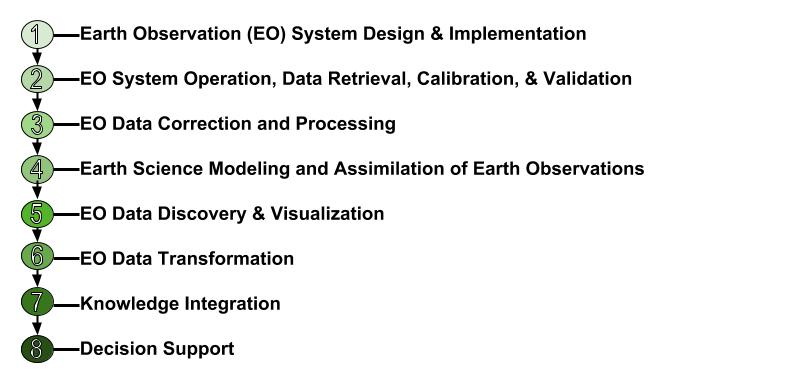
\includegraphics[width=0.7\textwidth]{Figures/chap7/EOChain.jpg}
    \caption{Generic Earth Observation Data Value Chain}
    \label{fig:eochain}
\end{figure}

\textbf{Conduct rapid prototyping \& co-design, without sacrificing stakeholder analysis.} In order to confirm that the proper data and dynamics are being captured, as well as to ensure the utility of the model to decision-makers and designers, the key stakeholders must be involved at all stages of the design process. Additionally, since most individuals have a difficult time providing concrete advice and criticism when discussing the abstract, rapid prototyping and mock-ups are important for stimulating feedback. One key component of this is always making sure that the user interface is available in the native language of the primary users.

Pursuing such rapid prototyping should not be allowed to cause the initial iteration of the \ac{saf} or the stakeholder analysis portion in particular to be sacrificed. Chapter \ref{ch:vida} did precisely this, resulting in a series of analyses and \ac{dss} components that were not as well connected to each other and to stakeholder needs as should have been the case.

\textbf{Enlist appropriate experts and stakeholders.} The design of any \ac{eo} system is inherently interdisciplinary and this is also true for \ac{eo} applications. For this reason the development necessarily involves a wide range of collaborators who vary both in terms of discipline (systems engineering, urban planning, earth science, economics, etc.) and it terms of institution (academic researchers, government officials, \ac{ngo} and corporate leaders, local activists, etc.). Rather than make assumptions when confronted with an issue outside our expertise, we must our utmost to recruit or consult with a relevant expert. 

A key part of this is recognizing that these experts and stakeholders will have their own perspectives and priorities that will not always align. This is one of the primary purposes of the \ac{saf}: to understand and synthesize these perspectives. But it is also important to recognize that, particularly if the \ac{evdt} moderator is outside of the target community, one must be intentional with how one aligns (or appears to align) with the various stakeholders. Finding a relatively neutral actor to serve as a primary Local Context Expert can be quite useful for enabling productive collaboration with a wide range of stakeholders, as can independently cultivating relationships with different stakeholders. This was done in the Chapter \ref{ch:mangroves} case study, for example. Other projects however call for a more clear declaration of one's stance, even if this risks alienating certain stakeholders.

\textbf{Maintain open access and modularity for adaptation and reuse, without overly sacrificing usability.} The intent is not for the \ac{evdt} Framework is not to develop complete, black-box products, but rather to facilitate the development of widely accessible \acp{dss}. Part of this includes the collaborative aspect of the \ac{evdt} Framework, but another part is making the code itself readily available online and designing the analyses and \ac{dss} to be as reusable as possible. This helps prevent the monopolization of information that characterized some of the technocratic excesses discussed in Chapter \ref{ch:theory}. It also helps to ensure that new \ac{evdt} projects may, for example, be able to reuse previous \ac{eo} data processing techniques, while focusing on the vulnerability or decision-making components.

At the same time, a rigid fixation on maximal open access and reusability should not be allowed to significantly detract from usability. The case studies from Chapters \ref{ch:mangroves} and \ref{ch:vida} perhaps ran amiss here, focusing too heavily on custom, open source, desktop-based \acp{dss} that limited there ability to be easily accessed and used by stakeholders with a wide range of technical competence. This can be contrasted with Jaffe's online \ac{dss}, which saw wider use \cite{jaffeEnvironmentalEconomicSystems2022}. Such cloud-based and internet-hosted tools can eliminate the need to direct possession of high performance computing equipment by either the end users or the developers. This reduces cost-of-entry for potential developers of \ac{evdt} models and ensures that end users can interact with, critique, and apply the models wherever they are, provided they have internet access. In general, implementers of future \ac{evdt} projects should, during the \ac{saf} process, be particularly attentive to existing decision-making processes of different stakeholders and design the \ac{dss} to fit well within them.

\textbf{Beyond technical open access, develop \ac{evdt} terminology, figures, and materials that are more inclusive of a non-technical audience.} One of the lessons of Section \ref{sec:lessons-foundational} was that a tension exists between the utility of technical fields and their accessibility to a wide set of stakeholders. This definitely applies to \ac{evdt} Framework, which has a highly technical-sounding name (and quite a bit of technical terminology within it). As discussed in Section \ref{sec:language}, it is important to adjust language based on the stakeholder to avoid exclusion. I certainly did precisely this during the case studies presented in this work, rarely using the term \ac{evdt} or other technical terminology when speaking to non-academic stakeholders, focusing instead on much more concrete and directly relevant matters instead. This is true of the other Space Enabled \ac{evdt} practitioners as well. 

Nonetheless, all of the publications on \ac{evdt} to date and almost all of the ancillary materials generated (outside of the \acp{dss} themselves) have been aimed at a technical audience. Moving forward, it would behoove us to document how we speak about the framework with non-technical stakeholders and us this to build up a corpus of more accessible materials. Figure \ref{fig:evdt_public} is an initial step in this direction, but a great deal more could be done. Other items could include a simplified how-to manual and case study summaries. These could broaden the appeal of the \ac{evdt} Framework (or whatever more accessible name is chosen for it) in a much more scalable fashion than having active practitioners explain it in understandable language to interested parties (as is currently done).

\textbf{Seek to build relationships and collaboration across \ac{evdt} projects.} One of the key findings of the Vida case study in Chapter \ref{ch:vida} was that there is significant utility in providing venues for communication and collaboration across study areas or even across \ac{evdt} projects. Some of these benefits are to the \ac{evdt} projects themselves, identifying potential new topics of analysis or providing opportunities for the re-use of code and other assets across projects. Some of these benefits are outside of the \ac{evdt} projects themselves but still quite useful in their own right. These can include peer-to-peer learning and instruction on other sustainable development topics.
 

\section{Advancing Stakeholder-Involved Sustainable Development Decision-making}

This dissertation presented a new framework for supporting sustainable development decision-making. The goal of the research was to demonstrate both the need for and the usefulness of this framework, and to thereby advance sustainable development action, particularly on the local scale. To address these goals, I undertook three main research efforts. First, I conducted a critical analysis of a variety of fields relevant to sustainable development (including the concept of sustainable development itself) to identify potential points of synergy and how to avoid historical pitfalls. Second, I built upon this analysis to develop the \acf{evdt} Framework. Third, I demonstrated the framework in two case studies, one a rather straightforward application and one a significant deviation that still contained useful lessons. In pursuing these case studies, I also provided useful analyses and tools to stakeholders.

As might be expected for a project of this scope, I did encounter challenges. Some of these challenges were internal to each case study and involved such things as the availability of data and understanding of the dynamics of the underlying phenomena. Some were part of the implementation, including a failure to conduct detailed usability studies or an urgency-and-complexity-based divergence from the \ac{evdt} Framework. Both provided useful lessons and the opportunity for future work.

It is my hope that the work presented in this thesis, I helped to fulfill a need for a generalized framework that combined multidisciplinary model integration, stakeholder participation and collaboration on a local scale, and the significant use of remote observation data for sustainable development. More broadly, I hope that this project serves to bridge the gap between disciplines (such as systems engineering and urban planning) and between stakeholders (such as academics, government officials, and members of the public) as we jointly try to pursue a more just and sustainable world.


